\section{Introduction}
\showtoc

%\subsection{Motivation}

\begin{frame}[t]
  \frametitle{Motivation}
  \begin{block}{Main Goal}
    Develop methods for improving the robustness of controllers for hybrid
    mechanical systems by shaping energy.
  \end{block}
    \begin{columns}
    \begin{column}{.333\textwidth}
      \begin{figure}
        \centering
        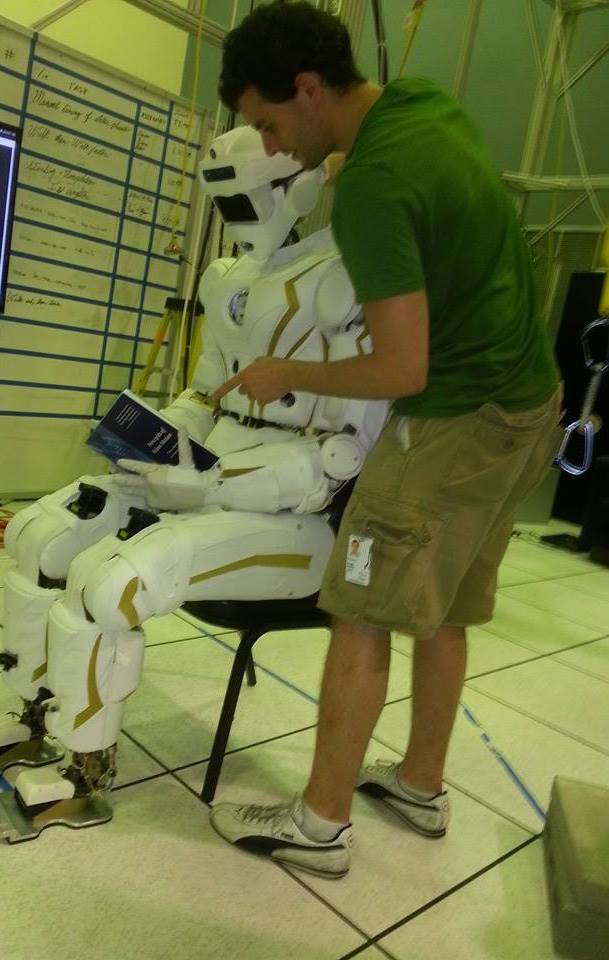
\includegraphics[height=4.0cm]{sinnet_valkyrie}
      \end{figure}
    \end{column}
    \begin{column}{.333\textwidth}
      \begin{figure}
        \centering
        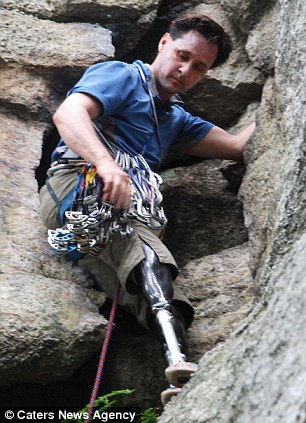
\includegraphics[height=4.0cm]{hugh_herr_climbing}
      \end{figure}
    \end{column}
    \begin{column}{.333\textwidth}
      \begin{figure}
        \centering
        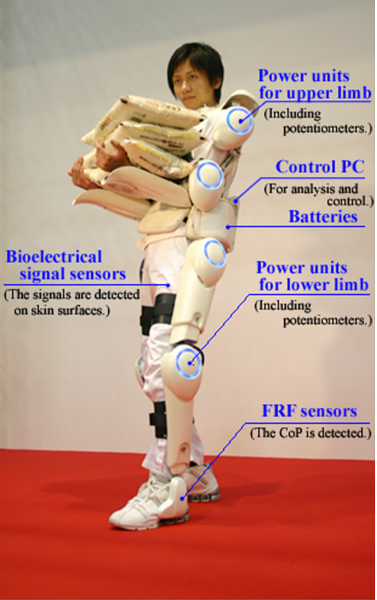
\includegraphics[height=4.0cm]{exoskeleton}
      \end{figure}
    \end{column}
  \end{columns}
\end{frame}

\begin{frame}[t]
  \frametitle{Summary of Accomplishments}
  \begin{itemize}
  \item NSF Graduate Research Fellowship in 2010
  \item 14 publications, 9 first author, 3 under review
  \item Co-authored featured survey article in Automatica
  \item Worked on DARPA Robotics Challenge, NASA--JSC team
  \item Award for Outstanding Student Research @ TAMU
  \item Travel awards from GSC and IROS
  \end{itemize}
\end{frame}
